\documentclass{thesis}
%%%%%%%%%%%%%%%%%%%%%%%%%%%%%%%%%%%%%%%%%%%%%%%%%%%%%%%%%%%%%%%%%%%%%%%%%%%%%%%%
% REQUIRED PACKAGES
%%%%%%%%%%%%%%%%%%%%%%%%%%%%%%%%%%%%%%%%%%%%%%%%%%%%%%%%%%%%%%%%%%%%%%%%%%%%%%%%
\usepackage{a4wide}
\usepackage{enumitem}

\usepackage{tabto}
\usepackage[T1]{fontenc}
\usepackage[utf8]{inputenc}
\usepackage[ngerman]{babel}
\usepackage{ae,aecompl}
\usepackage{ae}
\usepackage{graphicx}
\usepackage{bibgerm}
% \usepackage{mathptmx} %Schriftart Times New Roman

\usepackage{dsfont}
\usepackage{wrapfig}
\usepackage{afterpage}

\usepackage{subfigure}
\usepackage{caption}
\usepackage{fancyhdr}

\usepackage{amssymb}
\usepackage{amsmath}
\usepackage{amsfonts}

\usepackage{makeidx}
\usepackage{nomencl}
\usepackage{hyperref}
\usepackage{float}
\usepackage{color}
\usepackage[dvipsnames]{xcolor}
\usepackage{listings} %zur Einbindung von anderen Codes

\usepackage{braket}
\usepackage{url}

% \usepackage[style=chicago-authordate,natbib=true,backend=biber]{biblatex}
% for german language type 'ngernman' as option for babel package in in preamble.tex

%%%%%%%%%%%%%%%%%%%%%%%%%%%%%%%%%%%%%%%%%%%%%%%%%%%%%%%%%%%%%%%%%%%%%%%%%%%%%%%%
% PDF SETTINGS
%%%%%%%%%%%%%%%%%%%%%%%%%%%%%%%%%%%%%%%%%%%%%%%%%%%%%%%%%%%%%%%%%%%%%%%%%%%%%%%%

\hypersetup{
 pdfauthor={Luzian Uihlein},
 pdftitle={Extraktion von Diagrammen aus Texten und Auswertung von Liniendiagrammen mit Deep-Learning Methoden},
 pdfsubject={Not set},
 pdfkeywords={Not set}
}
\hypersetup{hidelinks} % hides boxes around hyperlinks uncomment this with ctrl+shift+7

%%%%%%%%%%%%%%%%%%%%%%%%%%%%%%%%%%%%%%%%%%%%%%%%%%%%%%%%%%%%%%%%%%%%%%%%%%%%%%%%
% BEGIN DOCUMENT
%%%%%%%%%%%%%%%%%%%%%%%%%%%%%%%%%%%%%%%%%%%%%%%%%%%%%%%%%%%%%%%%%%%%%%%%%%%%%%%%
\begin{document}



\begin{titlepage}
    \centering \mbox{}
    \large Bachelorarbeit \vfill  \Huge \textbf{Extraktion von Diagrammen aus Texten und Auswertung von Liniendiagrammen mit Deep-Learning Methoden} \\ \vfill \vfill \Large Luzian Uihlein \\ \vfill Würzburg, \today \\ \vfill \begin{figure}[h!] \begin{center} \includegraphics[height=8cm]{uni-siegel2.eps}
        \end{center}
    \end{figure}
    %\vfill

    Julius-Maximilians-Universität Würzburg \\
    Lehrstuhl für Informatik \RN{6}\\
    Betreuer: Prof. Dr. Frank Puppe\\
    \phantom{Betreuer: }Norbert Fischer\phantom{aaaaaa}\\
    \phantom{Betreuer: }Alexander Hartelt\phantom{aaaa}
\end{titlepage}

\thispagestyle{empty}
\cleardoublepage

\chapter*{Abstract}
\label{ch:abstract}

Diese Arbeit befasst sich mit der Erkennung von Diagrammen aus Texten, angewandt auf historische Wirtschaftsmagazine, sowie der automatischen Transkription von Liniendiagrammen. Durch die Entwicklung verschiedener Objekterkennungsmodelle wird die Erkennung und Klassifizierung von Diagrammtypen evaluiert. Für die Wertelinienerkennung der Liniendiagramme werden sowohl Instanzsegmentierung als auch semantische Segmentierung implementiert und verglichen. In Verbindung mit optischer Zeichenerkennung wird ein System zur Auswertung von Liniendiagrammen entworfen und bewertet. Die Ergebnisse zeigen, dass die Verwendung eines spezialisierten Algorithmus zur Digitalisierung von Diagrammdaten vielversprechend ist.

\renewcommand{\baselinestretch}{1} % decrease line spacing
\tableofcontents
\renewcommand{\baselinestretch}{1.2}

\normalsize

\chapter{Einleitung}
\label{ch:einleitung}

Die zunehmende Digitalisierung von Archivmaterialien ermöglicht es, historische Daten in einem nie dagewesenen Umfang zugänglich zu machen. Insbesondere die Massenextraktion und numerische Auswertung von Informationen aus historischen Dokumenten bieten ein enormes Potenzial für die Forschung. Diese Arbeit befasst sich mit der automatisierten Extraktion und Auswertung von Diagrammen aus Scans historischer Wirtschaftsmagazine. Ziel ist es, Methoden zu entwickeln und zu evaluieren, die eine automatische Massenerfassung numerischer Daten aus diesen Dokumenten ermöglichen.
\\
Im Fokus dabei steht die Extraktion verschiedener Diagrammarten aus Textscans und die anschließende Tabellenformauswertung extrahierter Liniendiagramme. Diese oft handgezeichneten und qualitativ unterschiedlichen Diagramme stellen eine besondere Herausforderung für die automatisierte Verarbeitung dar. Durch den Einsatz unterschiedlicher Deep-Learning-Methoden und speziell erstellter Datensätze wird die Effizienz der Extraktion und die Genauigkeit der daraus transkriptionierten Daten analysiert.
\\
Dabei werden verschiedene Aufgabenbereiche der maschinellen Bildverarbeitung erforscht. Für die Diagrammextraktion aus den Texten werden Objekterkennungs- und Klassifikationsmodelle trainiert. Die Liniendiagrammauswertung dagegen wird durch eine Kombination traditioneller Bildbearbeitungsmethoden, optischer Schriftzeichenerkennung und Bildsegmentierungsmodellen erforscht, wobei die Effizienz dieser ebenfalls anhand semantischer und Instanzsegmentierung verglichen wird.
\\
Die Arbeit gliedert sich in mehrere Abschnitte, die von der grundlegenden Datenaufbereitung über die Diagrammextraktion bis hin zur Auswertung der Liniendiagramme reichen. Ziel ist es, eine robuste Methode zur Massenextraktion und -auswertung zu entwickeln, die zukünftig als Grundlage für weiterführende Studien zur Analyse historischer Wirtschaftsdaten dienen kann.

\chapter{Literaturübersicht}
\label{ch:literaturübersicht}

Die automatische Transkription von Liniendiagrammen ist weit weniger erforscht als die von Tabellen, z.B. gibt es auf den ICDAR-Konferenzen (International Conference on Document Analysis and Recognition) keine Wettbewerbe (Challenges) mit annotierten Datensätzen, im Gegensatz zu Tabellen und vielen anderen Bereichen. Es gibt nur wenige Publikationen, die sich mit diesem Problem beschäftigen, wobei aktuelle Ansätze \cite{P2023LineEXDE, lee2023matgdmaterialsgraphdigitizer} Deep-Learning-Techniken verwenden, die mangels annotierter realer Daten überwiegend mit synthetischen Daten trainiert werden. In der Literatur wird die Erkennung von Liniendiagrammen meist in folgende Schritte unterteilt:

\begin{enumerate}[itemsep=0pt, topsep=0pt]
    \item Erkennen und Klassifizieren des Diagramms
    \item Erkennen der x- und y-Achse des Liniendiagramms
    \item Erkennen der Linien
    \item Erkennen der Beschriftungen
    \item Extraktion der Datenpunkte auf den Linien
    \item Zuordnung der Datenpunkte zu den semantischen x- und y-Werten
    \item Darstellung des Ergebnisses als Tabelle.
\end{enumerate}
% (1) Erkennen und Klassifizieren des Diagramms, (2) Erkennen der x- und y-Achse des Liniendiagramms, (3) Erkennen der Linien, (4) Erkennen der Beschriftungen, (5) Extraktion der Datenpunkte auf den Linien, (6) Zuordnung der Datenpunkte zu den semantischen x- und y-Werten, (7) Darstellung des Ergebnisses als Tabelle. 
Während einfache Linien gut erkannt werden, wird bei überlappenden Linien oft angenommen, dass diese farbig gezeichnet werden, um sie zu unterscheiden. Dies gilt jedoch nicht für historische Liniendiagramme, die in der Regel durch verschiedene gestrichelte Linien unterschieden werden, was automatisch schwer zu erkennen ist. Dafür eignen sich semiautomatische Ansätze wie z.B. in \cite{inproceedings} beschrieben. Hierbei werden die automatischen Schritte von den Anwendern sofort manuell überprüft und korrigiert, was bei einer Massentranskription nicht praktikabel, aber bei einer begrenzten Anzahl von Diagrammen realistisch ist, zumal eine Qualitätskontrolle für die GT-Erstellung ohnehin notwendig ist.
\\
Erforschte Herangehensweisen \cite{9423395} zur Linienerkennung und Datenextraktion bestehen unter anderem aus der Erkennung von Schlüsselpunkten (key point detection) der jeweiligen Wertelinien, welche hier durch Steigungsänderungen (pivot points) festgelegt werden. Nach deren Erkennung durch ein neurales Netzwerk werden diese mit Hilfe einer zusätzlichen Faltungsschicht (convolution layer) zu einzelnen Linieninstanzen gruppiert. Andere Linieninstanzgruppierungsalgorithmen \cite{parsingimages} bestehen in der Optimierung einer Kostenfunktion mithilfe der linearen Programmierung über ein Minimum-Kosten-Fluss-Problem (minimum-cost-flow problem). Im Vergleich zu handgeschriebenen, historischen Liniendiagrammen allerdings, bestehen die Datensätze exklusiv aus computergenerierten Textbeschriftungen, sodass die optische Schriftzeichenerkennung (optical character recognition) erfolgreicher durchgeführt werden kann. Die Zuordnung der Datenpunkte zu den semantischen x- und y-Werten erfolgt dadurch fehlerfreier, was wie bei allen Zwischenschritten die Effizienz des Endergebnisses direkt beeinflusst.
\\
Zur Evaluation werden die Linien als kontinuierliches Ähnlichkeitsproblem (continuous similarity problem) behandelt. Die Punktsequenz der Vorhersage des Modells und eine definierte Grundwahrheitsmenge werden verglichen, sodass Präzision (precision), Erinnerung (recall) und F1-Wert (F1-Score) berechnet werden können.

\chapter{Methodik}
\label{ch:methodik}

\section{Extraktion von Diagrammen aus Texten}

Ziel des ersten Teils ist die Extraktion der Diagrammen aus den historischen Textscans, welche dann im folgenden Teil in eine gewünschte Form ausgewertet werden können.
\\
Die Wesentlichen Schritte des Extraktionsteils beinhalten die Objekterkennung, also die Bestimmung des Begrenzungsrechtecks (bounding box) der Diagrammen innerhalb den vorliegenden Vollseitscans und deren Unterscheidung in verschiedene Diagrammtypen, beispielsweise Linien- und Balkendiagrammen.
Die erkannten Liniendiagramme werden anschließend anhand ihrer Auswertungsschwierigkeit klassifiziert, etwa durch Kennzeichnung deren Diagrammen, welche kontextbedingt gruppiert wurden, zum Beispiel aufgrund gemeinsamer Graphsachsen.

% \subsection{Erkennung von Diagrammen in Texten}
Um mit Hilfe von Deep-Learning Modelle zu trainieren, werden annotierte Grundwahrheiten (ground truth) benötigt.

\subsection{Datensatz DocBank zur Objekterkennung}

Für die Erkennung von Diagrammen in Texten wurden DocBank \cite{li2020docbank} und ein Anteil der historischen Wirtschaftsscans verwendet. DocBank besteht aus wissenschaftliche Publikation mit computergenerierten Grafiken zusammengesetzt, weshalb DocBanks Dokumentenseiten lediglich zum Vortrainieren des Detektionsmodells gedacht sind. Beabsichtigt wurde dieser Prozess des Vortrainierens um das System schneller und algemeingültiger, also mit besseren Voraussagen, trainieren zu können. Spätere Experimente untersuchen diese Annahme.
\\
An die Vorkommenshäufigkeit bei den historischen Scans angepasst, wurde die Differenzierung in fünf Objektklassen beschlossen: Linien (line), Balken (bar), Histogramm (histogram), Sonstige (other) und Gemischt (mixture). Aufgrund von Verwechslungen des Modells im Verlauf der Experimente zwischen Balkendiagrammen und Histogrammen wurden die Datensätze auf vier Klassen reduziert, indem Balkendiagramme und Histogramme vereinigt wurden.
\\
Die Schwierigkeit zwischen Balkendiagrammen und Histogrammen zu unterscheiden beruht darauf, dass Balkendiagramme kategorische Datenvergleiche anschaulich machen, bei denen die Balkenanordnung irrelevant ist, während Histogramme kontinuierliche, numerische Daten darstellen. Die Differenz liegt lediglich an der Achsenbeschreibung und nicht an visuellen Hinweisen, oftmals werden Balkendiagramme jedoch mit Lücken zwischen den Balken dargestellt, während Histogramme lückenlos abgebildet werden; dies ist allerdings nicht ausschlaggebend zur Bestimmung des Diagrammtyps.
\\
Für die manuell GT-Annotation der DocBank Dokumentenseiten, sowie folgender anderer Datensätze, wurde die Annotationssoftware CVAT \cite{CVAT_ai_Corporation_Computer_Vision_Annotation_2023} verwendet.

\begin{figure}[H]
    \centering
    \captionsetup{width=.75\linewidth}
    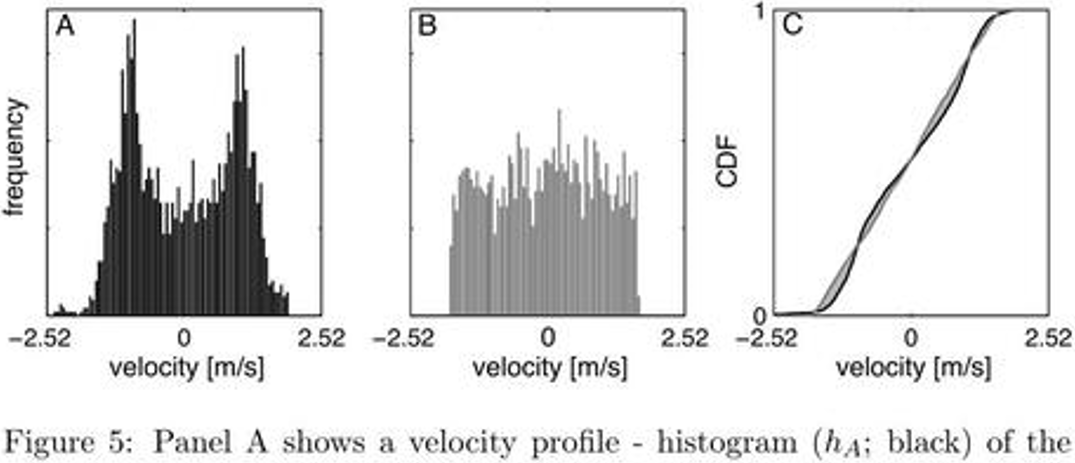
\includegraphics[width=.75\textwidth]{Methodik/img/docbank_example.png}
    \caption{\hbadness=10000 Beispiel kontextbedingter Gruppierung wegen gemeinsamer Y-Achsenbeschreibung eines gemischten Diagrammtyps (Histogramm und Liniendiagramm)}
    \label{fig:docbank_example}
\end{figure}

Da der Datensatz aus einer beträchtlich diversen Menge verschiedener wissenschaftlichen Publikationen besteht, beinhalten diese auch zahlreich verschiedene Diagrammlayouts. Um eine bestmögliche Konsitenz und Nützlichkeit in der Handannotation zu gewährleisten wurden einige Überlegungen gemacht: Da einige Abbildungen als Gruppe von Diagrammen fungieren, siehe Abbildung \ref{fig:docbank_example}, muss die generelle Entscheidung getroffen werden, jedes Diagramm der Gruppe einzeln zu annotieren oder lediglich die gesamte Gruppe zusammen. Beide Möglichkeiten liefern Vor- und Nachteile; beim getrennten Annotieren muss die Gruppe in einem späteren Schritt nicht mehr in die einzelnen Diagramme aufgeteilt werden, jedoch können auch kontextbedingte Informationen verloren gehen, wie in dem abgebildeten Beispiel die Y-Achsenbeschreibung des mittleren Diagramms (B), welches sich eine gemeinsame Y-Achsenbeschriftung mit dem linken Diagram (A) teilt.
Ebenfalls können Diagrammgruppen aus verschiedenen Diagrammtypen bestehen, etwa Histogramme und Liniendiagramme beieinander, weswegen dementsprechend für genau diesen Fall die gemischte Diagrammklasse eingeführt wurde. Bei weiteren Unklarheiten des Gruppenumfangs wurde sich sonst immer an die darunterliegenden Abbildungsunterschrift gehalten.
\\
Insgesamt wurden 321 Seiten annotiert, beinhaltend aus 105 Liniendiagrammen, 115 Balkendiagrammen (vereinigt mit Histogrammen), 79 sonstige und 66 gemischte Diagrammen.

\subsection{Datensatz historischer Wirtschaftsscans zur Objekterkennung}

\begin{wrapfigure}{r}{0.25\textwidth}
    \vspace{-\intextsep} % Remove vertical space above the figure
    \centering
    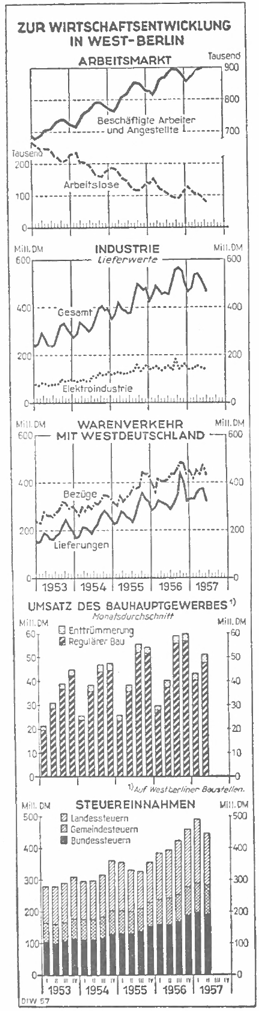
\includegraphics[width=\linewidth]{Methodik/img/scanbank_example.png}
    \caption{\hbadness=10000 Diagrammbeispiel historischer Scans}
    \label{fig:scanbank_example}
\end{wrapfigure}

Die Scans der geschichtlichen Wirtschaftsmagazine wurden mit ähnlichen Überlegungen annotiert. Hier befinden sich ebenfalls Diagrammgruppen, teils auch mit mehreren verschiedenen Diagrammtypen, siehe Abbildung \ref{fig:scanbank_example}, welche alle wieder als gesamte Gruppe annotiert wurden. Bis auf sehr wenigen Ausnahmen, befinden sich alle Abbildungen in den Scans visuell eingerahmt. Da die Ausrichtung derer jedoch nie wirklich perfekt gerade dargestellt wurde, und somit, der Ausrichtung verschuldet, kein Annotationsrechteck mit ausgeschlossenem Abbildungsrahmen gezeichnet werden kann wurde die Entscheidung getroffen, jede Annotation mit allen Ecken der Diagrammrahmen zu beinhalten. Grunsätzlich wurden alle Abbildungen, Diagramme oder nicht, wie etwa vereinzelte Karikaturen oder Landedskarten mit in die Klasse der sonstigen Diagramme eingeschlossen um so die allgemeine Erkennung von seltenen Diagrammtypen zu verstärken.
Es wurden insgesamt 2391 zufällige Seiten ausgewählt und manuell annotiert, woraus sich 343 Liniendiagramme, 102 Balkendiagramme, 77 sonstige und 52 gemischte Diagramme ergebten.

\clearpage
\section{Schwierigkeitsklassifizierung von Liniendiagrammen}

Aufgrund der überwiegenden Liniendiagrammen in den historischer Wirtschaftsscans, wurde sich im Folgenden primär auf die Auswertung der Liniendiagrammen fokusiert.
\\
Für genau diese Auswertung wurde der Vorverarbeitungsschritt überlegt, die extrahierten Liniendiagramme in verschiedene Untergruppen zu unterteilen. Es wurden vier Klassifikationen gewählt; Liniendiagramme mit nur einer Wertelinie, aus zusammengesetzten Diagrammen, also Liniendiagrammsgruppen, sich nicht überlappenden Wertelinien und sich überlappenden Wertelinien.

\begin{figure}[H] % or any other figure positioning (H, h, t, b)
    \centering
    \begin{minipage}{0.475\textwidth} % First figure
        \centering
        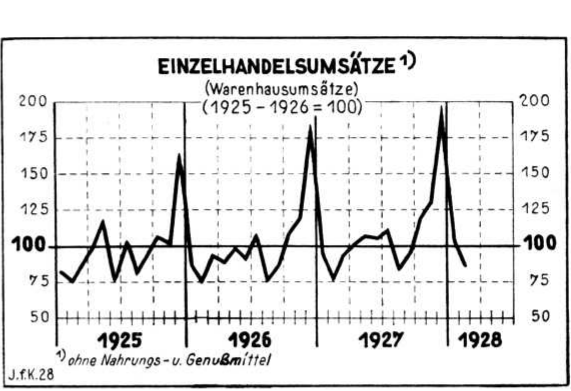
\includegraphics[width=\linewidth]{Methodik/img/linebank_single.png}
        \caption{\hbadness=10000 Liniendiagramm mit einer Wertelinie}
        \label{fig:linebank_single}
    \end{minipage}\hfill % Add space between figures
    \begin{minipage}{0.475\textwidth} % Second figure
        \centering
        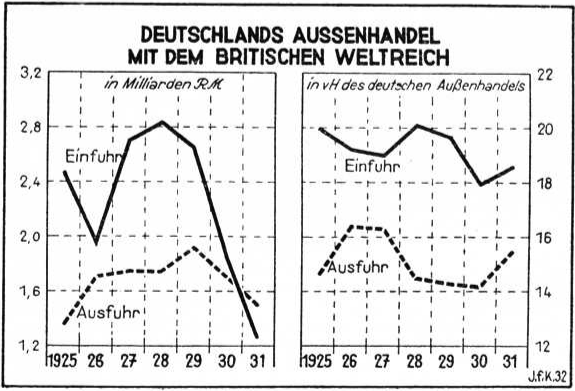
\includegraphics[width=\linewidth]{Methodik/img/linebank_composite.png}
        \caption{\hbadness=10000 Zusammengesetzte Liniendiagrammsgruppe}
        \label{fig:linebank_composite}
    \end{minipage}

    \vspace{0.75em}

    \begin{minipage}{0.475\textwidth} % First figure
        \centering
        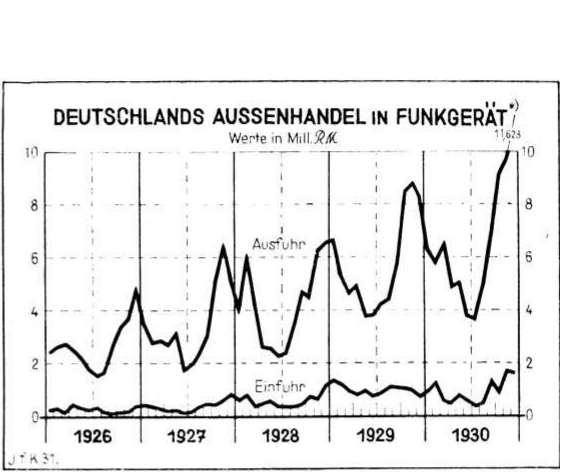
\includegraphics[width=\linewidth]{Methodik/img/linebank_non_overlapping.png}
        \caption{\hbadness=10000 Liniendiagramm mit sich nicht überlappenden Wertelinie}
        \label{fig:linebank_non_overlapping}
    \end{minipage}\hfill % Add space between figures
    \begin{minipage}{0.475\textwidth} % Second figure
        \centering
        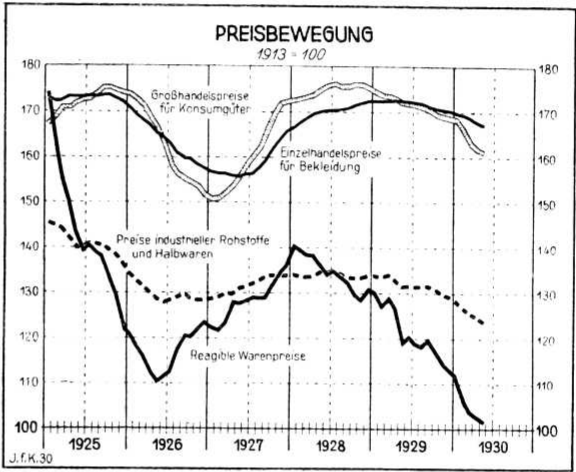
\includegraphics[width=\linewidth]{Methodik/img/linebank_overlapping.png}
        \caption{\hbadness=10000 Liniendiagramm mit sich überlappenden Wertelinie}
        \label{fig:linebank_overlapping}
    \end{minipage}
\end{figure}
Es existieren nämlich Liniendiagrammsgruppen mit mehreren eigenständigen Unterdiagrammen, welche möglicherweise jeweils ihre eigene Achsenbeschreibung haben, oder auch sich kontextbedingt diese Achsenbeschriftungen teilen. Diese müssen also im Vergleich zu einfachen Liniendiagrammen speziell behandelt werden. Aber auch wenn für Liniendiagramme mit nur einer oder sich nicht überschneidenden Wertelinien ein eher primitiver Extraktionsalgorithmus ausreichen würde, tritt bei komplexeren, sich überlappenden oder überschneidenden Wertelinien schnell das Problem der Linientrennung bzw. Liniengruppierung auf.
\\
Der erstellte Datensatz für die Schwierigkeitsklassifizierung besteht aus 807 klassifizierten Liniendiagrammen, unterteilt auf 93 mit einer Wertelinie, 284 zusammengesetzte, 94 nicht überlappendene und 336 überlappende Liniendiagramme.

\section{Auswertung von Liniendiagrammen}

Für die Auswertung der historischen Liniendiagramme wurden Überlegungen gemacht, Beschriftungen und vorallem das Hintergrundgitter, welches sich in jedem Diagramm zu finden lässt, zu entfernen, jedoch wurde schnell klar, dass diese primitive Herangehensweise grundsätzlich eher impraktibel ist. Zum einen führen die nicht genau senkrecht und waagerecht verlaufenden Gitterlinien die korrekte Erkennung dieser zu einem nichttrivialem Erkennungsproblem und zum andern überlappen und verlaufen viele Wertelinien auf dem Gitter, sodass die einfache Entfernung der Gitterlinienpixel das Diagramm mit unzähligen Lücken verbleiben lässt. Dementsprechend wurde beschlossen, statt aus dem Diagramm alles bis auf die Wertelinien zu entfernen, die Wertelinien selbst zu extrahieren, also sie durch Segmentation vom Hintergrundgitter und allen anderen Elementen zu trennen.
\\
Die manuelle Erstellung der Grundwahrheiten für die Werteliniensegmentation ist allerdings recht arbeitsaufwendig, weswegen zusätzlich ein synthetisch erstellter Datensatz generiert wurde, bei dem die Erstellung von Binärmasken der Wertelinien trivial ausfällt.
\\
Im Folgenden wird die Datensatzerstellung für die sowohl semantischer Segmentation, als auch Instanzsegmentation beschrieben. Die semantische Segementation benötigt pro Klasse nur eine gemeinsame Binärmaske, unabhängigt von der Anzahl der Objekte, also in dem Fall der Werteliniensegmentation eine Maske pro Liniendiagramm. In dem Fall der Instanzsegmentation dagegen, wird nicht nur eine eigene Maske pro jeweiliges Objektaufkommen - pro Objektinstanz - erfordert.

\clearpage

\subsection{Datensatz von synthetischen Liniendiagrammen zur Segmentation}

\begin{figure}[H] % or any other figure positioning (H, h, t, b)
    \centering
    \begin{minipage}{0.475\textwidth} % First figure
        \centering
        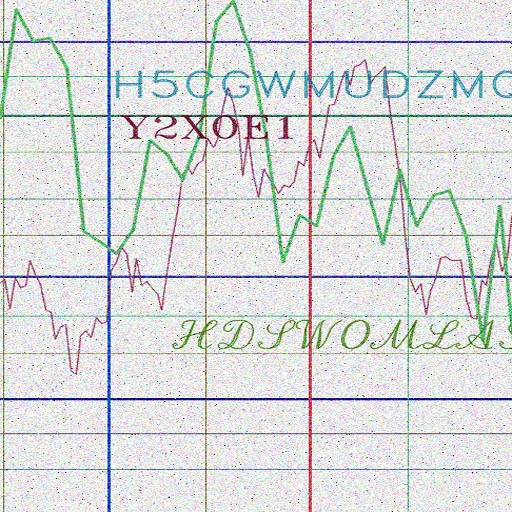
\includegraphics[width=\linewidth]{Methodik/img/lines_synthetic.png}
        \caption{\hbadness=10000 Synthetisch erstelltes Liniendiagramm}
        \label{fig:lines_synthetic}
    \end{minipage}\hfill % Add space between figures
    \begin{minipage}{0.475\textwidth} % Second figure
        \centering
        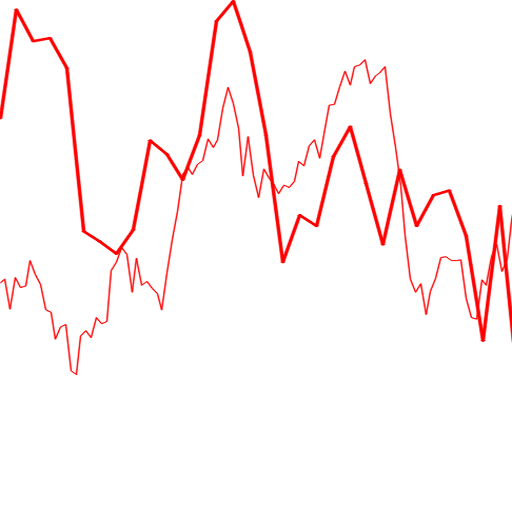
\includegraphics[width=\linewidth]{Methodik/img/lines_synthetic_mask.png}
        \caption{\hbadness=10000 Zugehörige generierte Binärmaske der Wertelinien}
        \label{fig:lines_synthetic_mask}
    \end{minipage}
\end{figure}

Der synthetische Datensatz besteht aus 2000 verschiedenen, zufällig generierten Liniendiagrammen. Diese beinhalten zufällige Wertelinien und Gitterlinien, sowohl in Position als auch in Liniendicke und beliebige, teils den Wertelinien überlappenden, Textbeschriftungen vielfältiger Schrifgrößen und Schriftarten. Da beim Generierungsprozess alle Diagrammswerte natürlicherweise bekannt sind, können diese einfach auf einem zweiten, leeren Bild übertragen werden, um so die zugehörige Wertelinienbinärmaske der semantischen Segmentation zu erstellen. Für die Instanzsegmentation dagegen, können diese auf getrennte Bilder gezeichnet werden. Je nach Implementation werden oftmals auch keine Binärmasken bei der Instanzsegmentation verwendet, sondern stattdessen Annotation im Format von Polygonumzeichnungen. Ist dies der Fall, können die getrennten Wertelinienbinärmasken unter anderem mit Hilfe von Konturerkennung in das gewünschte Polygonannotationsformat gebracht werden. Nachbearbeitet wurden die generierten Liniendiagramme am Ende mit unterschiedlichem Bildrauschen, um so näher an die Scanqualität und Diversität der historischen Diagramme heranzukommen.

\clearpage

\subsection{Datensatz von historischen Liniendiagrammen zur Segmentation}

\begin{figure}[H] % or any other figure positioning (H, h, t, b)
    \centering
    \begin{minipage}{0.475\textwidth} % First figure
        \centering
        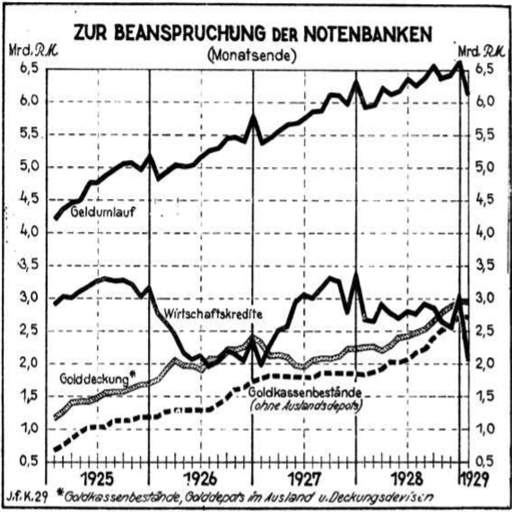
\includegraphics[width=\linewidth]{Methodik/img/lines_historical.png}
        \caption{\hbadness=10000 Historisches Liniendiagramm \phantom{Platzhalter}}
        \label{fig:lines_historical}
    \end{minipage}\hfill % Add space between figures
    \begin{minipage}{0.475\textwidth} % Second figure
        \centering
        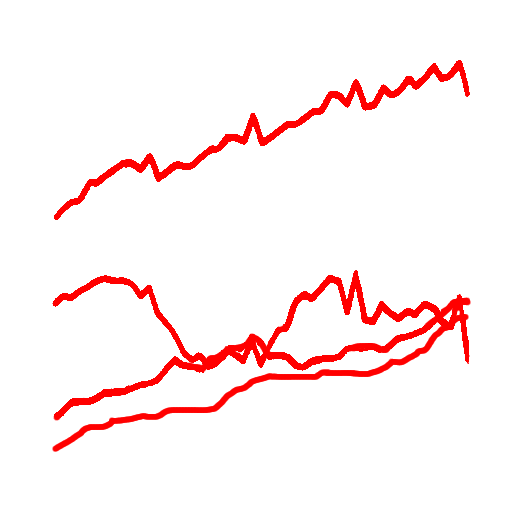
\includegraphics[width=\linewidth]{Methodik/img/lines_historical_mask.png}
        \caption{\hbadness=10000 Zugehörige manuell erstellte Binärmaske der Wertelinien}
        \label{fig:lines_historical_mask}
    \end{minipage}
\end{figure}

Die manuelle Erstellung der Wertelinienbinärmasken der historischen Liniendiagrammen fällt dagegen nicht ganz so leicht aus. Für die Anfertigung der Werteliniengrundwahrheiten wurde das Originalbild in einem Bildbearbeitungsprogramm \cite{photopea} geöffnet und pro Wertelinie eine eigene Bildschicht (layer) hinzugefügt. In jeder dieser einzelnen Schichten kann dann die jeweilige Wertelinine überzeichnet - abgepaust - werden. Der Grund jede Wertelinie in ihre eigene Maskenschicht zu übertragen ist der, dass am Ende einfach alle Schichten getrennt exportiert werden können. Für die semantische Segementation ist dies allerdings nicht nötig, da pro Klasse nur eine gemeinsame Binärmaske verwendet wird. Hier können jedoch dann ganz einfach alle exportierten Schichten in eine gemeinsame Maske vereinigt werden. In dem Fall der Instanzsegmentation dagegen wird eben nicht nur eine vereinigte Binärmaske pro Klase benötigt, sondern eine eigene Maske pro Objektinstanz - pro Wertelinie. Dementsprechend können hierfür die getrennten Maskenschichten verwendet werden. Werden hierfür wieder die Grundwahrheiten im Polygonannotationsformat erfordert, können diese, wie zuvor beschreiben, durch Konturerkennung von der Binärmask konvertiert werden.
\chapter{Implementation}
\label{ch:implementation}

\chapter{Experimente}
\label{ch:experimente}

Die verwendeten Metriken bei der Objekterkennung fassen sich aus Präzision (precision), Erinnerung (recall), mAP50 und mAP50-95 zusammen. Zum Berechnen dieser wird das Aufkommen der Richtig Positiven (TP), Falsch Positiven (FP) und Falsch Negativen (FN) Vorhersagen (predictions) des Modells benutzt. Die Kategorie TP zeigt vom Modell richtig erkannte Objekte, welche tatsächlich vorhanden sind, FP bestimmt die falsche Erkennung des Modells von Objekten die in Wirklichkeit nicht vorhanden sind und FN gibt Auskunft über Objekte die in der Realität vorhanden sind, das Modell sie allerdings nicht erkannt hat.
\\

Precision misst den Anteil der korrekten positiven Vorhersagen an allen positiven Vorhersagen des Modells. Sie zeigt, wie genau das Modell bei der Erkennung von Objekten ist und wie gut es falsche positive Ergebnisse vermeidet. Ein hoher Precision-Wert bedeutet, dass wenn das Modell ein Objekt erkennt, es mit hoher Wahrscheinlichkeit tatsächlich vorhanden ist.

\[Precision = \frac{TP}{TP + FP}\]
Recall misst den Anteil der korrekt erkannten positiven Instanzen an allen tatsächlichen positiven Instanzen. Es zeigt, wie gut das Modell alle vorhandenen Objekte einer Klasse findet. Ein hoher Recall-Wert bedeutet, dass das Modell die meisten der tatsächlich vorhandenen Objekte erkennt.

\[Recall = \frac{TP}{TP + FN}\]
mAP50 (mittlere durchschnittliche Präzision bei IoU=0.5) ist eine Metrik, die die Genauigkeit des Modells bei der Objekterkennung über alle Klassen hinweg misst. Dabei wird ein Intersection over Union (IoU) Schwellenwert von 0,5 verwendet. Eine Erkennung gilt als korrekt (TP), wenn die IoU zwischen der vorhergesagten und der tatsächlichen Bounding Box größer als 0,5 ist. Ein hoher mAP50-Wert zeigt, dass das Modell einfache Objekte verschiedener Klassen zuverlässig erkennt und lokalisiert.

\[mAP50 = \frac{1}{n} \sum_{i=1}^{n} AP_i\]
\emph{wobei $n$ die Anzahl der Klassen ist und $AP_i$ die durchschnittliche Präzision für die i-te Klasse bei IoU=0.5.}
\hbadness=10000\\\\
mAP50-95 (mittlere durchschnittliche Präzision bei IoU=0.5:0.95) ist eine umfassendere Metrik, die die Leistung des Modells über verschiedene IoU-Schwellenwerte hinweg misst. Sie berechnet den Durchschnitt der mAP-Werte für verschiedene IoU-Schwellenwerte von 0,5 bis 0,95 in Schritten von 0,05. Dies gibt einen robusteren Überblick über die Modellleistung, da es verschiedene Grade der Überlappungsgenauigkeit berücksichtigt. Ein hoher mAP50-95-Wert zeigt, dass das Modell sowohl bei einfachen als auch bei schwereren zuverlässige Vorhersagen trifft.

\[\mathit{mAP50\mbox{-}95} = \frac{1}{10} \sum_{t=0.5}^{0.95} mAP_t\]

\emph{wobei t die IoU-Schwellenwerte von 0.5 bis 0.95 in Schritten von 0.05 durchläuft.}
\hbadness=10000\\\\




Im Kapitel "Experimente" Ihrer Bachelorarbeit sollten Sie die durchgeführten Versuche, deren Ergebnisse und Ihre Analyse darlegen. Hier ist eine Übersicht der wichtigsten Punkte, die in diesem Kapitel enthalten sein sollten:

Versuchsaufbau:

Beschreibung der verwendeten Datensätze (Trainings-, Validierungs- und Testdaten)
Erklärung der Evaluierungsmetriken (z.B. mAP für YOLO, IoU für U-Net)
Definition der Baseline oder Vergleichsmodelle


Durchgeführte Experimente:

Detaillierte Beschreibung jedes einzelnen Experiments
Begründung für die Wahl der Experimente
Variationen in Hyperparametern, Modellarchitekturen oder Trainingsmethoden


Ergebnisse:

Präsentation der quantitativen Ergebnisse (in Tabellen oder Grafiken)
Qualitative Ergebnisse (z.B. Beispielbilder von Vorhersagen)
Vergleich der Leistung von YOLO und U-Net für Ihre spezifische Aufgabe


Analyse:

Interpretation der Ergebnisse
Diskussion von Stärken und Schwächen der Modelle
Vergleich mit dem aktuellen Stand der Technik oder anderen relevanten Arbeiten


Ablationstudie:

Untersuchung des Einflusses verschiedener Komponenten oder Hyperparameter auf die Modellleistung


Fehleranalyse:

Identifikation von häufigen Fehlertypen
Diskussion möglicher Gründe für diese Fehler


Laufzeitanalyse und Ressourcenverbrauch:

Vergleich der Inferenzzeiten von YOLO und U-Net
Analyse des Speicher- und Rechenbedarfs


Diskussion der Limitationen:

Grenzen der durchgeführten Experimente
Mögliche Verzerrungen in den Daten oder der Evaluation


Zukünftige Arbeiten:

Vorschläge für weitere Experimente oder Verbesserungen basierend auf Ihren Ergebnissen



Dieses Kapitel sollte eine objektive Darstellung Ihrer experimentellen Arbeit sein, die es dem Leser ermöglicht, die Leistung und Eignung von YOLO und U-Net für Ihre spezifische Anwendung zu verstehen und zu bewerten.
\chapter{Zusammenfassung}
\label{ch:zusammenfassung}

In dieser Arbeit wurde sich mit der Entwicklung und Evaluation eines Systems zur Massenextraktion verschiedener Diagramme in Texten und Auswertung von Liniendiagrammen aus historischen Wirtschaftsmagazinen beschäftigt. Hierfür wurde eine Kombination unterschiedlicher Deep-Learning-Techniken und traditioneller Bildbearbeitungsmethoden implementiert.
\\
Die experimentellen Ergebnisse zeigen, dass die gewählten Modelle vielversprechend für die automatische Extraktion und Klassifikation diverser Diagrammarten sind. Die semantische Segmentation der Wertelinien von Liniendiagrammen erwies sich als robuster im Vergleich zur Instanzsegmentation mit Ultralytics YOLO, insbesondere bei der korrekten Erkennung aller vorliegenden Wertelinien. Die Vereinigung der Segmentierungsergebnisse mit optischer Schriftzeichenerkennung für die Achsenbestimmung ermöglichte die grafische Darstellung und numerische Auswertung in Tabellenform.
\\
Allerdings gibt es auch Limitationen, die in zukünftigen Arbeiten weiter ausgearbeitet werden können. Durch das Wegfallen der Linieninstanzerkennung bei semantischer Segmentation wurde ein simpler Linientrennungsalgorithmus entwickelt, welcher bei komplexeren, insbesondere bei sich überlappenden Linien von Diagrammen zu Fehlern führt. Hierfür könnten Kombinationen aus semantischer und Instanzsegmentation oder sogar ganz andere erforschte fortschrittlichere Liniennachzeichnungs- oder Gruppierungsalgorithmen zu verbesserten Ergebnissen führen. Zudem ist die vorgeschlagene Methode stark von der Qualität der optischen Schriftzeichenerkennung abhängig, weshalb hierfür verschiedene OCR-Bibliotheken oder auf historischen Dokumenten spezialisiert trainierte OCR-Modelle evaluiert werden könnten.
\\
Insgesamt bieten die entwickelten Methoden eine solide Grundlage für die weitere Forschung im Bereich der automatisierten Diagrammerkennung und -auswertung. Zukünftige Arbeiten könnten sich ebenfalls auf die Generalisierbarkeit dieser Methoden auf andere Diagrammarten konzentrieren.

\appendix

\bibliographystyle{unsrt}
\bibliography{refs}

\fancyhf{}
\renewcommand{\headrule}{}

\begin{center}
\LARGE \textbf{Declaration of originality}\normalsize
\end{center}

\bigskip

I declare that I have authored this thesis independently, that I have not used other than the declared sources / resources, and that I have explicitly marked all material which has been quoted either literally or by content from the used sources.

\setlength{\bigskipamount}{5em}
\bigskip

Würzburg, \today \hfill Name Name ......................................



% \let\clearpage\relax


%table of figures
%\clearpage
%\listoffigures
%\clearpage

%empty page 
% \thispagestyle{empty}
% \cleardoublepage

\phantom{
    \cite{P2023LineEXDE}
    \cite{lee2023matgdmaterialsgraphdigitizer}
    \cite{inproceedings}
    \cite{9423395}
    \cite{parsingimages}
    \cite{li2020docbank}
    \cite{CVAT_ai_Corporation_Computer_Vision_Annotation_2023}
    \cite{photopea}
    \cite{Jocher_Ultralytics_YOLO_2023}
    \cite{ronneberger2015unetconvolutionalnetworksbiomedical}
    \cite{redmon2016lookonceunifiedrealtime}
    \cite{lin2015microsoftcococommonobjects}
    \cite{dwyer2024roboflow}
    \cite{chollet2015keras}
    \cite{info11020125}
    \cite{opencv_library}
    \cite{zak2024kerasunet}
    \cite{kingma2017adammethodstochasticoptimization}
    \cite{dimden2024chromelensocr}
    \cite{Hunter:2007}
    \cite{2020SciPy-NMeth}
    \cite{DamianoP2024confusionMatrixGenerator}
}

\end{document}


